%------------------------------------------------------------------------
% Chapter:  Quickstart
%------------------------------------------------------------------------

\chapter{Quick start \label{quick}}

In order to quickly illustrated the usage of {\it PDFFIT} for those
impatient readers, a PDF refinement of $Ni$ will be illustrated. The
data used here were collected at room temperature using the diffractometer
at beamline X7A at NSLS, Brookhaven National Laboratory. The data are
terminated at $Q_{max}=22$\AA$^{-1}$. The data as well as the resulting
PDF are shown as filled circles in Figure \ref{quick-fig1}.

\begin{figure}[!b]
   \centering
   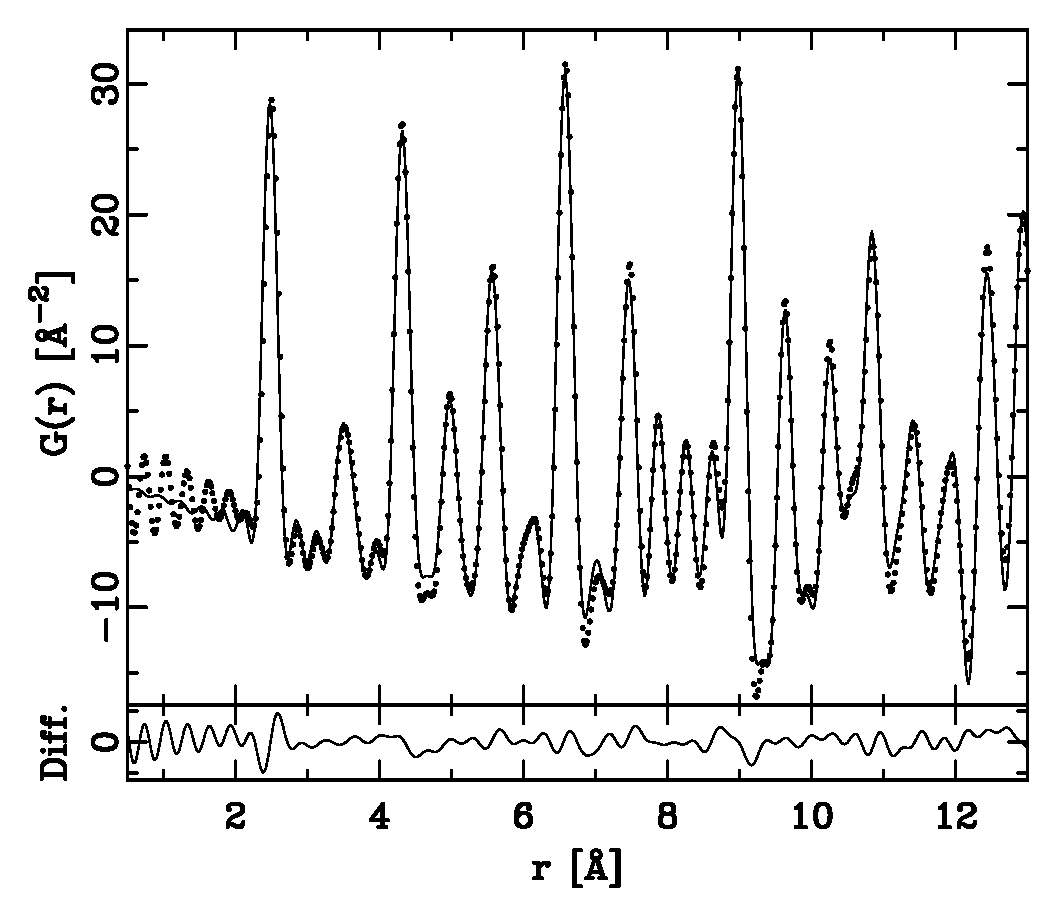
\includegraphics[scale=0.6, angle=0.0]{quick.1.eps}
   \caption[Result of PDF refinement of $Ni$]
           {Result of PDF refinement of $Ni$. The solid line is the
            calculated PDF, the filled circles are the data. A difference
            curve is plotted below the data.}
   \label{quick-fig1}
\end{figure}

The sequence of commands used to carry out the refinement is listed
below. Note that the line numbers are only added for easy reference and
are not actually part of the input. The commands can either be written
using a text editor and executed as macro file of typed in at the
{\it PDFFIT} command prompt.

\footnotesize
\begin{MacVerbatim}
      1 reset
      2 read stru,ni.stru
      3 read data,x,22.0,0.0,ni.data
      4 #
      5 par lat[1]=p[1],1.0
      6 par lat[2]=p[1],1.0
      7 par lat[3]=p[1],1.0
      8 #
      9 do i[1]=1,n[1]
     10   par u[1,i[1]]=p[2],1.0
     11   par u[2,i[1]]=p[2],1.0
     12   par u[3,i[1]]=p[2],1.0
     13 enddo
     14 #
     15 par csca[1]=p[10],1.0
     16 par qsig[1]=p[11],1.0
     17 par delt[1]=p[12],1.0
     18 #
     19 p[1]=lat[1]
     20 p[2]=u[1,1]
     21 #
     22 p[10]=1.50
     23 p[11]=0.03
     24 p[12]=0.10
     25 #
     26 range 1,0.5,13.0
     27 run
     28 #
     29 save pdf,1,ni_ref.calc
     30 save dif,1,ni_ref.dif
     31 save stru,1,ni_ref.stru
     32 save res,ni_ref.out
\end{MacVerbatim}
\normalsize

\noindent The command {\tt reset} in line 1 resets {\it PDFFIT} to
have a defined initial state. Next a structural model (line 2) and
the experimental PDF (line 3) are read. The format of these text
files are discussed in section \ref{file} of this manual. The
parameters of the command {\tt read data} are the radiation type
(here X-ray), $Q_{max}$ and the resolution factor $\sigma_{Q}$
associated with the data file '{\it ni.data}'. {\it PDFFIT} allows
the user to freely define relations between structural and
experimental parameters and the refinement parameters {\tt p[i]}.
This is done using the command {\tt par}. The lattice parameters
$a,b,c$ are stored in {\it PDFFIT} variables {\tt lat[1], lat[2]}
and {\tt lat[3]}. In lines 5--7 of the example above refinement
parameters {\tt p[1]} is used to refine all three lattice
parameters since $Ni$ is cubic and $a=b=c$. The additional
parameter {\tt 1.0} is the derivative of the parameter on the left
with respect to the refinement parameters. These derivatives are
needed for the least-squares refinement (see Appendix
\ref{app-deriv} for details). In our case we have a simple one to
one correspondence and the derivative is trivial. In lines 9--13
the temperature factors $U_{lm}$ of the atoms are associated with
a single refinement parameter {\tt p[2]}. Note that we have four
$Ni$ sites in our model and rather than typing the definitions for
each atom separately, we are using a loop. Details about loops and
variables are given in section \ref{fort}, all we need to know for
now is that the variable {\tt n[1]} contains the number of sites.
In our example we only refine an isotropic temperature factor, so
we use the same parameter for $U_{11}, U_{22}$ and $U_{33}$ stored
in {\tt u[1,n], u[2,n]} and {\tt u[3,n]}. Next we associate
individual refinement parameters with the scale factor $f_{p}$
(line 15), the resolution factor $\sigma_{Q}$ (line 16) and the
dynamic correlation factor $\delta$ (line 17). Note that there is
no need for a consecutive numbering of the parameters. Finally we
need to initialize the refinement parameters {\tt p[i]} with
suitable starting values which is done in lines 19--24. Last we
define the $r$-range we want to use for the refinement (line 26),
here from 0.5\AA\ to 13.0\AA. The argument of the {\tt range}
command is the number of the dataset (see section \ref{fit_mult}).
There is generally no predefined order for the commands, however,
data need to be read first and obviously all desired settings must
be entered before the refinement is started using the command {\tt
run} (line 27). The screen output during the refinement is shown
below:

\footnotesize
\begin{MacVerbatim}
     Starting refinement ...
     --------------------------------------------------------------------------
     Iteration  :   0  Sum:  48995.5     Urf:  1.00798
                       R  : 0.155190     Rw : 0.154659
     Parameters :
       1:  3.52032       2: 0.515471E-02  10:  1.50000      11: 0.300000E-01
      12: 0.100000
     --------------------------------------------------------------------------
     Iteration  :   1  Sum:  44646.7     Urf:  1.00165
                       R  : 0.148137     Rw : 0.147636     DRw: -.702314E-02
     Parameters :
       1:  3.51974       2: 0.505564E-02  10:  1.48549      11: 0.313635E-01
      12: 0.127834
     --------------------------------------------------------------------------
     Iteration  :   2  Sum:  44352.0     Urf:  1.00089
                       R  : 0.147658     Rw : 0.147148     DRw: -.488088E-03
     Parameters :
       1:  3.52014       2: 0.501998E-02  10:  1.48752      11: 0.319241E-01
      12: 0.131231
     --------------------------------------------------------------------------
     Iteration  :   3  Sum:  49266.2     Urf:  1.00054
                       R  : 0.155582     Rw : 0.155086     DRw: 0.793780E-02
     Parameters :
       1:  3.52056       2: 0.501416E-02  10:  1.48125      11: 0.286770E-01
      12: 0.135971
     --------------------------------------------------------------------------
\end{MacVerbatim}
\normalsize

\noindent For each iteration the program prints $\sum
(G_{obs}-G_{calc})^{2}$ ({\tt sum}), the R-value ({\tt R}), the
weighted R-value ({\tt Rw}) and the difference of the R-value
compared to the previous cycle ({\tt DRw}). Furthermore the actual
values of all refinement parameters {\tt p[i]} are listed. Note
that iteration 3 has a slightly higher R-value compared to
iteration 2, so the refinement converged or exploded depending on
the size of the (now positive) difference. The resulting
parameters correspond actually to the output of the $(n-1)$th
cycle. However, the display of the iteration that lead to the
termination of the refinement might help to judge how well the fit
converged. \par

In lines 29--32 we have to save the resulting PDF, the difference between
observed and calculated PDF, the resulting structure and
fit results, respectively. The calculated PDF can be plotted using
e.g. {\it KUPLOT} which is part of the {\it DISCUS} software package.
Figure \ref{quick-fig1} was generated using {\it KUPLOT}. The final
structure can also be exported in {\it DISCUS} format for further
analysis. \par

After this quick run through a quite simple example refinement we will
discuss all features of the program {\it PDFFIT} in more detail.
Additionally the command reference and the online help of the program
might be a valuable source of information. Use the command {\tt help}
when in {\it PDFFIT} to activate the online help facility of the
program.

%------------------------------------------------------------------------
